


\numberwithin{equation}{section}






\section{Deep Convolutional Neural Fields}


In this Appendix, we show some technical details about the proposed deep convolutional field model.





Let $\x$ be an image and $\y=[y_1,\ldots, y_n]^{\T} \in \Real^n$ be
%the continuous real-valued vectorized depth map of
a vector of continuous depth values corresponding to
 all $n$ superpixels in $\x$.
 %Continuous \crf (CCRF)
 Similar to conventional CRF,
 we model the conditional probability distribution of the data with the following density function:
\begin{equation}\label{eq:prob}
\begin{aligned}
\Pr(\y|\x) = \frac{1}{\mathrm{Z}(\x)} \exp \{ -E(\y, \x) \},
\end{aligned}
\end{equation}
where $E$ is the energy function and $Z(\x)$ the partition function, defined respectively as:
\begin{equation}\label{eq:feature}
E(\y, \x) = \sum_{p \in {\cal N} } (y_p - \regress_p)^2
+ \sum_{(p,q) \in {\cal S}} \half \pws_{pq} (y_p - y_q)^2,
\end{equation}
\begin{equation}\label{eq:partition}
\mathrm{Z}(\x) = \int_{\y} \exp \{ -E(\y, \x) \}\mathrm{d}\y,
\end{equation}
in which,
\begin{equation} \label{eq:def_R}
\pws_{pq} = \sum_{k=1}^K \beta_k S_{pq}^{(k)},
\end{equation}
where $\regress$ is the regressed depths parametrized by $\btheta$ (namely, $\regress$ is the abbreviation of $\regress(\btheta)$), $\bbeta=[\beta_1, \ldots, \beta_K]$ the pairwise parameter, $\S^{(k)}$ the $k$-th similarity matrix (which is symmetric) and $K$ the number of pairwise terms considered.
To guarantee $Z(\x)$ (Eq. \eqref{eq:partition}) is integrable, $\bbeta_k > 0$ are required.
We aim to jointly learn $\regress(\btheta)$ and $\bbeta$ here.


By expanding Eq. \eqref{eq:feature}, we then have:
\begin{align} \label{eq:feature_expand}
E(\y, \x) &= \sum_p y_p^2 - 2\sum_p y_p \regress_p  + \sum_p \regress_p^2 + \half \sum_{pq} \pws_{pq} y_p^2 - \sum_{pq} \pws_{pq} y_p y_q + \half \sum_{pq} \pws_{pq} y_q^2 \notag \\
	&= \y^\T \y - 2\bregress^\T \y  + \bregress^\T \bregress +  \y^\T \D \y -  \y^\T \bpws \y  \notag \\
	&= \y^\T (\I+ \D - \bpws) \y - 2\bregress^\T \y + \bregress^\T \bregress \notag \\
	&= \y^\T \A \y - 2\bregress^\T \y + \bregress^\T \bregress,
\end{align}
%\bd = 2\regress
%\underbrace{(2\I+2\bbeta \D -2\bbeta \S)}_\text{\Sigma^{-1}}
where
\begin{align} \label{eq:def_A}
\A = \I+ \D - \bpws.
\end{align}
Here, $\I$ is the n$\times$n identity matrix; $\D$ is a diagonal matrix with $\D_{pp} = \sum_q \pws_{pq}$.
Since $\beta_k \geq 0$ are enforced, $\A$ is ensured to be positive definite ($\A$ is symmetric, and strictly diagonally dominant with positive diagonal entries). We can then calculate the partition function according to the Gaussian integral formula as:
\begin{align} \label{eq:part_expand}
Z(\x) &=\int_\y \exp \Big\{ -E(\y, \x) \Big\}\mathrm{d}\y   \notag \\
	&=  \int_{\y} \exp \Big\{ - \y^\T \A \y + 2\bregress^\T \y - \bregress^\T \bregress \Big\}\mathrm{d}\y  \notag  \\
	&=\exp \{  - \bregress^\T \bregress \} \int_{\y} \exp \Big\{ - \y^\T \A \y + 2\bregress^\T \y \Big\}\mathrm{d}\y \notag  \\
	&= \exp \{  - \bregress^\T \bregress \}\sqrt{\frac{{(2\pi)}^n}{|2\A|}} \exp \{{ \bregress ^\T \A^{-1} \bregress}\} \notag  \\
	&= \frac{{(\pi)}^{\frac{n}{2}}}{{|\A|}^{\frac{1}{2}}} \exp \{{ \bregress ^\T \A^{-1} \bregress   - \bregress^\T \bregress }\} ,
\end{align}
where $|\A|$ denotes the determinant of the matrix $\A$, and $\A^{-1}$ the inverse of $\A$.
From Eq. \eqref{eq:prob}, \eqref{eq:feature_expand}, \eqref{eq:part_expand}, we can write the probability density function as:
\begin{align} \label{eq:prob_gaussian}
\Pr(\y|\x) &=\frac{\exp \Big\{ -E(\y, \x) \Big\}} { Z(\x)}  \\ \notag
	&= \frac{\exp \Big\{ - \y^\T \A \y + 2\bregress^\T \y - \bregress^\T \bregress \Big\}}{\frac{{(\pi)}^{\frac{n}{2}}}{{|\A|}^{\frac{1}{2}}} \exp \{{ \bregress ^\T \A^{-1} \bregress   - \bregress^\T \bregress }\}}  \\ \notag
	&=\frac{ |\A|^{\half}} {{\pi^{\frac{n}{2}}}} \exp \Big\{ - \y^\T \A \y + 2\bregress^\T \y -  \bregress ^\T \A^{-1} \bregress \Big\}. \\ \notag
\end{align}
%%
%
%
According to Eq. \eqref{eq:prob_gaussian}, we can then rewrite the negative log-likelihood $-\log\Pr(\y|\x)$ as:
\begin{align} \label{eq:log-likelihood}
-\log\Pr(\y|\x)&= \y^\T \A \y - 2\bregress^\T \y + \bregress ^\T \A^{-1} \bregress - \half\log(|\A|) + \frac{n}{2}\log(\pi).
\end{align}


%In learning, CCRF minimizes the negative conditional log-likelihood of the training data,
%\begin{equation} \label{eq:ccrf}
%(\btheta^{\star}, \bbeta^{\star}) = \argmin_{\btheta, \bbeta} -L(\btheta, \bbeta) = \argmin_{\btheta, \bbeta} -\sum_{i=1}^N \log\Pr(\y^{(i)} | \x^{(i)}; \btheta, \bbeta)
%\end{equation}
In learning, we minimizes the negative conditional log-likelihood of the training data. Adding regularization to $\btheta$, $\bbeta$, we then arrive at the final optimization:
\begin{align} \label{eq:ccrf_final}
\min_{\btheta, \bbeta \geq \zeros} &-\sum_{i=1}^N \log\Pr(\y^{(i)} | \x^{(i)}; \btheta, \bbeta) + \frac{\lambda_1}{2} \fnorm \btheta + \frac{\lambda_2}{2} \fnorm \bbeta,
\end{align}
where $\x^{(i)}$, $\y^{(i)}$ denote the $i$-th training image and the corresponding depth map; $N$ is the number of training images; $\lambda_1$ and $\lambda_2$ are weight decay parameters.



For the unary part,
here we calculate the partial derivatives of $-\log\Pr(\y|\x)$ with respect to $\theta_l$ (one element of the network parameters $\btheta$ for the unary part ). Recall that $\A = \I+ \D - \bpws$ (Eq. \eqref{eq:def_A}), $\A^{\T}=\A$, $(\A^{-1})^{\T}=\A^{-1}$, $|\A^{-1}|=\frac{1}{|\A|}$, we have:
\begin{align}  \label{eq:derive_z}
\frac{\partial \{ -\log\Pr(\y|\x)\} }{\partial \theta_l} &= \frac{\partial \{-2\bregress^\T \y + \bregress ^\T \A^{-1} \bregress\}}{\partial \theta_l}   \\ \notag
&= \frac{\partial \{-2\bregress^\T \y \} } {\partial \theta_l} + \frac{\partial \{ \bregress ^\T \A^{-1} \bregress\}}{\partial \theta_l}   \\ \notag
&= -2 \frac{\partial \{ \sum_p \regress_p y_p \} } {\partial \theta_l} + \frac{\partial \{ \sum_{pq} \regress_p \regress_q A^{-1}_{pq} \}}{\partial \theta_l}   \\ \notag
&= -2 \sum_p \Big ( y_p\frac{\partial \regress_p } {\partial \theta_l} \Big ) + \sum_{pq} \Big ( z_p \frac{\partial  \regress_q} {\partial \theta_l} + z_q \frac{\partial  \regress_p} {\partial \theta_l} \Big ) A^{-1}_{pq} \\ \notag
&= -2 \y^{\T} \frac{\partial \bregress } {\partial \theta_l} + 2\bregress^{\T} \A^{-1} \frac{\partial \bregress } {\partial \theta_l}\\ \notag
&= 2 (\A^{-1} \bregress - \y)^{\T} \frac{\partial \bregress}{\partial \theta_l} .
\end{align}



%For the pairwise part, we first calculate the partial derivatives of $-\log\Pr(\y|\x)$ with respect to $\pws_{pq}$:
%\begin{align}  \label{eq:derive_R}
%\frac{\partial \{ -\log\Pr(\y|\x)\} }{\partial \pws_{pq}} &= \frac{\partial \{\y^\T \A \y + \bregress ^\T \A^{-1} \bregress - \half\log(|\A|)\}}{\partial \pws_{pq}}   \notag \\
%&= \frac{\partial \{ \y^\T \A \y \}}{\partial \pws_{pq}} +  \frac{\partial \{\bregress ^\T \A^{-1} \bregress\}}{\partial \pws_{pq}} - \half \frac{\partial \log(|\A|)}{\partial \pws_{pq}}, \notag \\
%&=\y^\T\frac{\partial  \A }{\partial \pws_{pq}}\y - \bregress^\T \A^{-1} \frac{\partial \A }{\partial \pws_{pq}} \A^{-1} \bregress  - \half \frac{1}{|\A|} \frac{\partial \{|\A|\} }{\partial \pws_{pq}}, \notag \\
%&=\y^\T \frac{\partial  \A }{\partial \pws_{pq}} \y - \bregress^\T \A^{-1} \frac{\partial \A }{\partial \pws_{pq}} \A^{-1} \bregress  - \half \trace \Big ( \A^{-1}  \frac{\partial \A} {\partial \pws_{pq}} \Big ), \notag \\
%&=\y^\T \G \y - \bregress^\T \A^{-1} \G \A^{-1} \bregress  - \half \trace \Big ( \A^{-1}  \G\Big ).
%\end{align}
%Here we introduce a matrix $\G=\frac{\partial  \A }{\partial \pws_{pq}}$. Each element of $\G$ is:
%\begin{align} \label{eq:def_G}
%G_{pq} &= \frac{\partial A_{pq} }{\partial \pws_{pq}}  \notag \\
%&= \frac{\partial \{  D_{pq} - \pws_{pq} \} }{\partial \pws_{pq}}  \notag \\
%%&= \frac{\partial \{  \sum_q \pws_{pq} - \pws_{pq} \} }{\partial \pws_{pq}}  \notag \\
%&= -\delta(p \neq q),
%\end{align}
%where $\delta(\cdot)$ is the indicator function, which equals 1 if $p \neq q$ is true and 0 otherwise.



Next, for the pairwise part, we calculate the  partial derivatives of $-\log\Pr(\y|\x)$ with respect to $\beta_k$ as:
\begin{align}  \label{eq:derive_beta}
\frac{\partial \{ -\log\Pr(\y|\x)\} }{\partial \beta_k} &= \frac{\partial \{\y^\T \A \y + \bregress ^\T \A^{-1} \bregress - \half\log(|\A|)\}}{\partial \beta_k}   \notag \\
&= \frac{\partial \{ \y^\T \A \y \}}{\partial \beta_k} +  \frac{\partial \{\bregress ^\T \A^{-1} \bregress\}}{\partial \beta_k} - \half \frac{\partial \log(|\A|)}{\partial \beta_k}, \notag \\
&=\y^\T\frac{\partial  \A }{\partial \beta_k}\y - \bregress^\T \A^{-1} \frac{\partial \A }{\partial \beta_k} \A^{-1} \bregress  - \half \frac{1}{|\A|} \frac{\partial \{|\A|\} }{\partial \beta_k}, \notag \\
&=\y^\T \frac{\partial  \A }{\partial \beta_k} \y - \bregress^\T \A^{-1} \frac{\partial \A }{\partial \beta_k} \A^{-1} \bregress  - \half \trace \Big ( \A^{-1}  \frac{\partial \A} {\partial \beta_k} \Big ).
\end{align}
We here introduce matrix $\J$ to denote $\frac{\partial  \A }{\partial \beta_k}$. Each element of $\J$ is:
\begin{align}  \label{eq:def_J}
J_{pq} &= \frac{\partial A_{pq}}{\partial \beta_k}  \notag \\
&= \frac{\partial \{ D_{pq} - R_{pq} \} }{\partial \beta_k}  \notag \\
&= \frac{\partial D_{pq}  }{\partial \beta_k}  - \frac{\partial R_{pq}  }{\partial \beta_k} \notag \\
&= - \frac{\partial  \pws_{pq} }{\partial \beta_k} + \delta(p=q) \sum_q \frac{\partial  \pws_{pq} }{\partial \beta_k},
\end{align}
where $\delta(\cdot)$ is the indicator function, which equals 1 if $p=q$ is true and 0 otherwise.
From Eq. \eqref{eq:derive_beta}, Eq. \eqref{eq:def_J}, we can see that our framework is general, therefore more complicated networks for the pairwise part can be seamlessly incorporated.
Here, in our case, with the definition of $\pws_{pq}$ in Eq. \eqref{eq:def_R}, we have $\frac{\partial  \pws_{pq} }{\partial \beta_k}=S_{pq}^{(k)}$.

According to Eq. \eqref{eq:derive_beta} and the definition of  $\J$ in \eqref{eq:def_J}, we can now write the partial derivative of $-\log\Pr(\y|\x)$ with respect to $\beta_k$  as:
\begin{equation}  \label{eq:derive_beta_final}
\frac{\partial \{ -\log\Pr(\y|\x)\} }{\partial \beta_k} =  \y^{\T} \J \y - \bregress^{\T} \A^{-1} \J \A^{-1}\bregress - \half \trace \Big( \A^{-1} \J \Big).
\end{equation}
%%
%Using the chain rule, we can write the partial derivatives of  $-\log\Pr(\y|\x)$ with respect to $\theta_l$ as:
%\begin{align}
%\frac{\partial \{ -\log\Pr(\y|\x) \} } {\partial \theta_l}
% = \; & \frac{\partial \{ -\log\Pr(\y|\x) \} }{\partial \bregress} \frac{\partial \bregress }{\partial \theta_l}   \notag \\
% = \; & \Big( 2 \A^{-1} \bregress - 2\y \Big ) \frac{\partial \bregress }{\partial \theta_l} , \label{eq:derive_z}
%\end{align}

\paragraph{Depth prediction}
Predicting the depths of a new image is to solve the MAP inference.
Because of the quadratic form of $\y$ in Eq. \eqref{eq:log-likelihood}, closed form solutions exist (details refer to supplementary): % \cite{ccrf_nips08}:
\begin{align} \label{eq:inf_solution1}
\y^{\star}&=\argmax_{\y} \Pr(\y|\x)  \notag \\
&=\argmax_{\y} \log \Pr(\y|\x) \notag   \\
&= \argmax_{\y} -\y^\T \A \y + 2\bregress^\T \y .
\end{align}
With the definition of $\A$ in Eq.\eqref{eq:def_A}, $\A$ is symmetric.
Then by setting the partial derivative of $-\y^\T \A \y + 2\bregress^\T \y$ with respect to $\y$ to $\zeros$ ($\zeros$ is an n$\times$1 column vector with all elements being 0), we have
\begin{align} \label{eq:inf_deriv}
&\frac{\partial \{ -\y^\T \A \y + 2\bregress^\T \y \} } {\partial \y} =0  \notag  \\
\Rightarrow \;\;&-(\A + \A^{\T} ) \y +2 \bregress=0  \notag  \\
\Rightarrow \;\;&-2\A \y +2 \bregress=0  \notag  \\
\Rightarrow \;\;&\y = \A^{-1} \bregress.
\end{align}
Now we can write the solution for the MAP inference in Eq. \eqref{eq:inf_solution1} as:
\begin{align} \label{eq:inf_solution2}
\y^{\star}&= \A^{-1} \bregress
\end{align}

%Because of the quadratic form of $\y$ in Eq. \eqref{eq:log-likelihood}, there exists closed form solution for the inference problem \cite{ccrf_nips08}:
%\begin{equation} \label{eq:inference}
%\y^{\star}=\argmax_{\y} \Pr(\y|\X) = \argmax_{\y} -\y^\T \A \y + 2\regress^\T \y  = \A^{-1} \regress.
%\end{equation}
%If the pairwise terms are ignored, namely $\bbeta=\zeros$, then Eq. \eqref{eq:inference} degenerates to $\y^{\star}=\regress$, which is a conventional regression model.




\section{Experiments}
To show how the superpixel number affects the performance of our model, we add an experiment to evaluate the root mean square (rms) errors and the training time of our pre-train model on the Make3D dataset by varying the superpixel number per image.
Fig. \ref{fig:rmsVSspnum} shows the results.
As we can see, increasing the number of supperpixel per image yields further decrease in the rms error, but at the cost of more training time.
We use $\sim 700$ superpixels per image in all other experiments in this paper, therefore by increasing it, we can expect better results.


\begin{figure} \center
     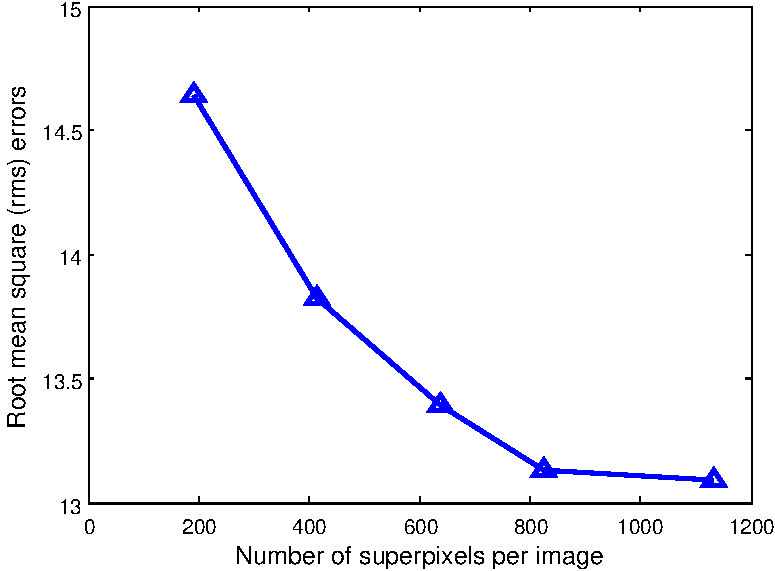
\includegraphics[width=0.38\textwidth, height=0.28\textwidth]{./fig/Make3D/rmsVSspNum.pdf}
     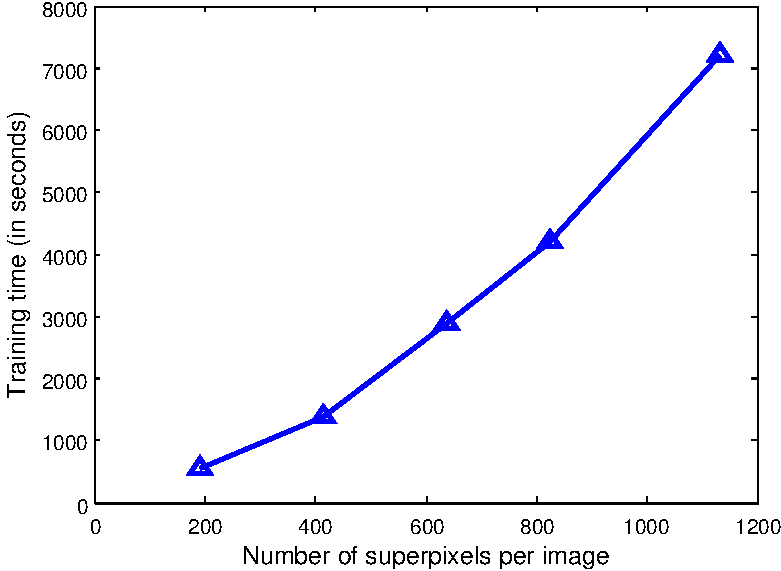
\includegraphics[width=0.38\textwidth, height=0.28\textwidth]{./fig/Make3D/timeVSspNum.pdf}
\caption{Left: Root mean square (C2 rms)  errors  \vs  varying superpixel numbers on the Make3D dataset.
Right: Training time \vs varying superpixel numbers per image on the Make3D dataset.
Clearly, increasing the number of supperpixels per image, we can further improve the results but at the cost of more training time.}  \label{fig:rmsVSspnum}
\end{figure}


